\chapter{Kiến thức nền tảng}
\ifpdf
\graphicspath{{Chapter2/Chapter2Figs/PNG/}{Chapter2/Chapter2Figs/PDF/}{Chapter2/Chapter2Figs/}}
\else
\graphicspath{{Chapter2/Chapter2Figs/EPS/}{Chapter2/Chapter2Figs/}}
\fi
\label{chap_2}
\begin{quote}
	
	\textit{Trong chương này, chúng tôi sẽ trình bày những kiến thức nền tảng trên ba chủ đề bao gồm: mô hình ngôn ngữ, mạng nơ-ron hồi quy và Long short-term memory. Mô hình ngôn ngữ cho phép dự đoán từ tiếp theo trong một chuỗi từ cho trước; trong dịch máy, nó giúp tạo ra những bản dịch lưu loát. Mạng nơ-ron hồi quy (RNN) là xương sống của dịch máy nơ-ron. RNN được dùng làm bộ mã hóa lẫn bộ giải mã. Ứng với mỗi vai trò, RNN sẽ có một thiết kế riêng. Long short-term memory (LSTM) là phiên bản cải tiến của RNN nhằm giải quyết vấn đề về phụ thuộc dài hạn. LSTM cũng là phiên bản RNN được dùng để xây dựng nên Bộ mã hóa - Bộ giải mã trong khóa luận này. Những thành phần nói trên cung cấp kiến thức nền tảng để đi đến mô hình dịch máy nơ-ron theo kiến trúc Bộ mã hóa - Bộ giải mã mà chúng tôi sẽ trình bày trong chương 3}.
	
\end{quote}

\section{Mô hình ngôn ngữ}

Như đã nói trong chương 1, mô hình ngôn ngữ là thành phần không thể thiếu trong dịch máy; nó đảm bảo rằng hệ thống tạo ra những bản dịch "trơn tru" (fluent). Trong dịch máy nơ-ron, người ta thường sử dụng mô hình ngôn ngữ dựa trên mạng nơ-ron hồi quy (trong khóa luận này nó là một LSTM). Trước khi đi đến mô hình ngôn ngữ dựa trên mạng nơ-ron hồi quy, chúng tôi sẽ nhắc lại một vài mô hình ngôn ngữ đã được sử dụng trong quá khứ, cũng như những điểm mạnh, yếu của từng mô hình. Những đặc điểm ấy nói lên rằng vì sao mô hình ngôn ngữ dựa trên mạng nơ-ron hồi quy là hướng tiếp cận nổi bật và thích hợp cho bài toán dịch máy nơ-ron.

Mô hình ngôn ngữ là một phân phối xác suất trên một chuỗi các từ nhằm đánh giá độ trơn tru của chuỗi ấy so với những chuỗi khác. Cho trước một chuỗi $w_1,w_2,...,w_n$, mô hình ngôn ngữ gán cho nó một xác suất $p(w_1,w_2,...,w_n)$ đại diện cho độ trơn tru của chuỗi đó, ví dụ $p($"How tall are you ?"$) >$ $p($"How high are you ?"$)$ vì từ "high" trong thực tế không dùng để hỏi về chiều cao của con người. Theo công thức xác suất có điều kiện, ta có:
\begin{equation} \label{traditionalLM}
\begin{split}
p(w_1,...,w_n) &= p(w_1)p(w_2|w_1)p(w_3|w_1,w_2)...p(w_n|w_1,w_2,...,w_{n-1}) \\
&= \prod_{t=1}^{n} p(w_t|w_1,w_2,...,w_{t-1})
\end{split}
\end{equation}

Trong công thức trên, mỗi thành phần $p(w_i|w_1,w_2,...,w_{i-1})$ là xác suất có điều kiện của từ $w_i$ biết những từ trước đó $w_1,w_2,...,w_{i-1}$, những từ này còn được gọi là ngữ cảnh đối với từ đang xét. Nhận thấy rằng để tính được xác suất $p(w_i|w_1,w_2,...,w_{i-1})$ mô hình phải xét đến tất cả những từ đứng trước nó. Điều này làm cho chi phí tính toán trở nên rất lớn. Để giảm chi phí tính toán, người ta sử dụng giả định \textit{markov} (markov-assumption); giả định này nói rằng các từ tiếp theo chỉ liên quan đến từ hiện tại và độc lập với các từ trước đó. Chính xác hơn, một giả định markov bậc $k$ nói rằng từ tiếp theo trong một chuỗi chỉ phụ thuộc vào $k$ từ cuối cùng trong chuỗi.
\begin{equation} \label{markovAssumption}
p(w_{i+1}|w_1,w_2,...,w_{i}) \approx p(w_{i+1}|w_{i-k},..w_{i})
\end{equation}

Công thức \ref{traditionalLM} theo giả định markov trở thành:
\begin{equation} \label{traditionalLM2}
p(w_{1:n}) = \prod_{t=1}^{n} \approx p(w_{i-k}|w_{i-k},..w_{i-1})
\end{equation}

Mặc dù giả định markov bậc $k$ rõ ràng là sai với $k$ bất kỳ (một câu có thể có phụ thuộc dài hạn với chiều dài bất kỳ như câu bắt đầu bằng từ \textit{what} và kết thúc bằng dấu \textit{?}), tuy nhiên nó vẫn tạo ra những mô hình ngôn ngữ mạnh mẽ với với các giá trị tương đối nhỏ của $k$ ($k=3$ hoặc $k=5$), và là phương pháp chủ yếu cho bài toán mô hình hóa ngôn ngữ trong hàng thập kỷ.

Do mô hình ngôn ngữ là một mô hình học không giám sát, một cách thông thường để đánh giá một mô hình học không giám sát là áp dụng nó lên một bài toán học có giám sát rồi đánh giá thông qua kết quả của bài toán đó, ví dụ: đo lường sự cải thiện chất lượng dịch khi chuyển đổi từ mô hình ngôn ngữ A sang mô hình ngôn ngữ B trong một hệ thống dịch máy. Cách đánh giá này được gọi là đánh giá bên ngoài (extrinsic evaluation). Tuy nhiên, đánh giá bên ngoài rất tốn kém đối với những bài toán học có giám sát lớn và phức tạp. Vì vậy, một độ đo được thiết kế để đánh giá mô hình ngôn ngữ một cách nội tại (intrinsic evaluation) đó là perplexity. Perplexity là một độ đo để đánh giá một mô hình xác suất tốt như thế nào khi dự đoán một mẫu chưa nhìn thấy (unseen sample). Cho trước một tập ngữ liệu $ W = w_1, w_2, ..., w_N$ ($N$ là một số rất lớn) và một mô hình ngôn ngữ \textit{LM}, perplexity của $W$ ứng với mô hình ngôn ngữ \textit{LM} là:
\begin{equation} \label{perplexity}
\begin{split}
Perplexity(W) &= LM \left(p(w_1,...,w_N) \right)^{-\frac{1}{N}} \\
&= \sqrt[N]{\frac{1}{LM(p(w_1,...,w_N))}} \\
&= \sqrt[N]{\prod_{i=1}^{N}  \frac{1}{LM(p(w_i|w_1,...,w_{i-1}))}} \\
\end{split}
\end{equation}
%&= 2^{-\frac{1}{N} \sum_{i=1}^{N} \log_2 LM(p(w_i|w_1,...,w_{i-1}))}

Một mô hình ngôn ngữ tốt sẽ gán xác suất lớn cho những chuỗi trong tập ngữ liệu (phản ánh đúng ngôn ngữ thật sự) sẽ dẫn đến một giá trị nhỏ của perplexity và ngược lại. Trong công thức \ref{perplexity}, có thể nhìn thấy nếu xác suất của một chuỗi càng lớn thì perplexity càng nhỏ. Do đó, cực tiểu hóa perplexity cũng tương đương với việc cực đại hóa xác suất của chuỗi. Perplexity là một độ đo tốt và thuận tiện để đánh giá các mô hình ngôn ngữ với nhau, nhưng việc perplexity được cải thiện khi ta thay đổi mô hình ngôn ngữ không đảm bảo rằng đánh giá bên ngoài cũng được cải thiện. Tuy vậy, perplexity vẫn thường được sử dụng như là một cách kiểm tra nhanh một mô hình ngôn ngữ. 

Cách tiếp cận truyền thống cho bài toán mô hình hóa ngôn ngữ là sử dụng mô hình ngôn ngữ \textit{n}-gram. Sở dĩ nó có tên như vậy là vì nó sử dụng giả định markov bậc \textit{n} - 1 để ước lượng xác suất $p \left(w_{i+1}=m|w_1,..,w_i \right) \approx p \left(w_{i+1}=m|w_{i-(n-1)},...,w_i \right)$. Theo mô hình ngôn ngữ \textit{n}-gram, xác suất để từ $m$ theo sau chuỗi các từ $w_1,...,w_{i}$ là:

\begin{equation} \label{ngramLM}
p \left(w_{i+1}=m|w_{i-(n-1):i} \right) = \frac{\# \left(w_{i-(n-1)},...,w_{i+1} \right)}{\# \left(w_{i-(n-1)},...,w_i \right)}
\end{equation}
trong đó $\#(w_{i:j})$ là số lần xuất hiện của chuỗi $w_i,...,w_j$ trong tập ngữ liệu. Các mô hình \textit{n}-gram thông thường sử dụng $n = 3$ và $n = 2$ được gọi lần lượt là mô hình \textit{trigram} và mô hình \textit{bigram}. Trong trường hợp mô hình không sử dụng ngữ cảnh để ước lược lượng xác
suất của một từ ($n = 0$), thì mô hình này được gọi là mô hình \textit{unigram}.

Mô hình ngôn ngữ \textit{n}-gram là một mô hình phi tham số, nó có một ưu điểm là tốc độ tính toán rất nhanh (do các xác suất của các \textit{n}-gram đã được tính toán trước và lưu trữ lại) và dễ dàng mở rộng cho nhiều lĩnh vực (ta chỉ cần tập ngữ liệu thuộc lĩnh vực ấy). Mặc dù có một vài mô hình ngôn ngữ có kết quả tốt hơn so với mô hình \textit{n}-gram, tuy nhiên các mô hình đó thường kèm theo độ phức tạp tính toán lớn và kết quả cải thiện không đáng kể. Do đó, mô hình \textit{n}-gram vẫn được sử dụng phổ biến cho đến ngày nay.

Mặc dù vậy, mô hình \textit{n}-gram vẫn còn nhiều hạn chế. Đầu tiên, mặc dù tốc độ tính toán của mô hình \textit{n}-gram là nhanh, nhưng kèm theo đó là sự đánh đổi về mặt lưu trữ. Nếu tập ngữ liệu là lớn thì mô hình phải lưu những bảng xác suất khổng lồ, điều này gây ra khó khăn khi ta muốn sử dụng mô hình này trên các thiết bị có bộ nhớ nhỏ như thiết bị di động hay cảm biến. Thứ hai, điểm yếu của mô hình này đến từ việc sử dụng giả định markov; giả định này khiến cho mô hình \textit{n}-gram không thể nắm bắt được các thông tin ngữ cảnh dài hạn. Ví dụ cho trước ngữ cảnh \textit{"Columbus is the man who discovered \_\_"}, ta muốn từ tiếp theo sẽ là \textit{"America"}; một mô hình \textit{5}-gram không thể dự đoán được từ tiếp theo là \textit{"America"} vì độ dài ngữ cảnh tối đa của nó chỉ đạt đến từ \textit{"is"}.

Thứ ba, ta thấy rằng trong mô hình \textit{n}-gram, nếu một chuỗi $\left(w_i,...,w_j \right) \subseteq w_1,...,w_n$ chưa từng xuất hiện trong tập ngữ liệu, tức $\# \left(w_i,...,w_j \right) = 0$ thì xác suất ước lượng $p(w_{j+1}|w_i,...,w_j)$ sẽ có giá trị bằng 0. Điều này dẫn đến xác suất của toàn bộ chuỗi $w_1,...,w_n$ cũng bằng 0 do phép nhân trong công thức tính của nó (công thức \ref{traditionalLM}). Việc xác suất bằng 0 xảy ra khá thường xuyên do sự giới hạn của tập ngữ liệu. Một cách để tránh việc xảy ra các sự kiện xác suất bằng không là sử dụng những kỹ thuật \textit{làm mịn} (smoothing techniques). Làm mịn bảo đảm tất cả mọi chuỗi đều có một xác suất xuất hiện (mặc dù nhỏ). Kỹ thuật làm mịn đơn giản nhất là làm mịn thêm $\alpha$ (add-$\alpha$ smoothing) \cite{goodman2001}; nó bảo đảm bất kỳ chuỗi nào cũng xuất hiện ít nhất $\alpha$ lần. Với làm mịn thêm $\alpha$ ta được:
\begin{equation} \label{ngramLMWithSmoothing}
p_{add-\alpha} \left(w_{i+1}=m|w_{i-k},...,w_{i} \right) = \frac{\# \left(w_{i-(n-1)},...,w_{i+1} \right) + \alpha}{\# \left(w_{i-(n-1)},...,w_{i} \right) + \alpha \left|V \right| }
\end{equation}
trong đó $\left|V \right|$ là số lượng từ vựng trong tập ngữ liệu. Hiện nay phương pháp làm mịn Kneser-Key là phương pháp phổ biến và đạt được kết quả tốt nhất \cite{jurafsky2000}.

Ngoài ra còn một vấn đề với mô hình \textit{n}-gram là \textbf{tính tổng quát hóa không cao} \cite{bengioLM2003}. Điều này có thể được giải thích bằng việc mô hình này coi các cụm từ là rời rạc khiến nó không có khả năng nắm bắt được tính tương tự về ngữ nghĩa giữa các từ \cite{bengioLM2003}. Xét hai câu sau: $s_1 =$ \textit{"She is a good cook"} và $s_2 =$ \textit{"She cooks very well"}, ta thấy rằng hai câu này về mặt ngữ nghĩa là tương đương nhau nên ta muốn xác suất của chúng cũng xấp xỉ nhau $p(s_2) \approx p(s_1)$. Tuy vậy, do một lý do nào đó mà câu $s_2$ xuất hiện ít hơn rất nhiều so với câu $s_1$ nên $p(s_2) \ll p(s_1)$. Do đó, có thể thấy rằng việc không nắm bắt tính tương tự về ngữ nghĩa làm cho mô hình ngôn ngữ \textit{n}-gram có tính tổng quát hóa không cao.

\begin{figure}
	\centering
	\includegraphics[width=0.5\textwidth]{wordembedding}
	\caption[Minh họa cách biểu diễn từ bằng word embedding]{Minh họa cách biểu diễn từ bằng word embedding: một từ $w_i$ được biểu diễn dưới dạng véc-tơ one-hot, $w_i$ sau đó được biến đổi thành $x_i$ dựa trên một phép biến đổi tuyển tính với ma trận $P$ của phép biến đổi. $|V|$ là số lượng từ vựng, $D_e$ là số chiều của word embedding được xác định trước.}
	\label{fig_wordembedding}
\end{figure}

Trong bài báo "A Neural Probabilistic Language Model" \cite{bengioLM2003}, giáo sư Yoshua Bengio và các cộng sự đã đề xuất một mô hình ngôn ngữ dựa trên mạng nơ-ron truyền thẳng. Nó giải quyết hai vấn đề mà mô hình \textit{n}-gram gặp phải: một là mô hình ngôn ngữ dựa trên mạng nơ-ron truyền thẳng là một mô hình tham số, nghĩa là đầu ra sẽ được tính dựa trên các tham số của mô hình sau khi được huấn luyện), điều này giúp giảm bộ nhớ lưu trữ - đặc biệt hơn những tham số này sẽ được chia sẻ cho toàn bộ mô hình, điều này giúp tăng tính tổng quát hóa \cite{bengioLM2003}; hai là nó sử dụng biểu diễn véc-tơ để biểu diễn các từ gọi là word embedding, điều này giúp mô hình có khả năng nắm bắt tính tương tự về ngữ nghĩa giữa các từ. Hình \ref{fig_wordembedding} mô tả cách tạo ra các véc-tơ embedding. Word embedding sẽ được nhắc lại một lần nữa trong mục \ref{wordembeddingsection}: Biểu diễn từ trong mạng học sâu.

Tuy nhiên, mô hình này vẫn dựa trên giả định markov. Tại mỗi thời điểm, đầu vào của mạng là một nối dài của các véc-tơ embedding tại những thời điểm trước đó $i_t = \left[ x_{t-(n-1)},...,x_t \right]$ trong đó $x_i$ là véc-tơ embedding của từ $w_i$, $n$ là bậc của giả định markov (hình \ref{fig_fnnlm} mô tả cách hoạt động của mô hình). Đây là một khuyết điểm lớn của mô hình khi nó chỉ nắm bắt được thông tin trong một vùng $n - 1$ từ trước đó. Do những khuyết điểm này, một mô hình ngôn ngữ dựa trên \textit{mạng nơ-ron hồi quy} được đề xuất trong \cite{mikolovLM}. Mô hình này kế thừa những ưu điểm của mô hình ngôn ngữ dựa trên mạng nơ-ron truyền thẳng và có khả năng nắm bắt được thông tin trên một vùng có chiều dài bất kỳ. Mô hình này sẽ được nói đến trong phần kiến thức cơ bản về mạng nơ-ron hồi quy và được giải thích chi tiết trong chương 3 trong mục bộ giải mã. 

\begin{figure}
	\centering
	\includegraphics[width=0.8\textwidth]{fnnlm}
	\caption[Minh họa mô hình ngôn ngữ dựa trên mạng nơ-ron truyền thẳng]{Minh họa mô hình ngôn ngữ dựa trên mạng nơ-ron truyền thẳng: mô hình nhận đầu vào là các véc-tơ ngữ cảnh $w_{t-(n-1)},...,w_t$ dưới dạng one-hot, sau đó những véc-tơ này được biểu diễn lại dưới dạng các véc-tơ embedding $x_{t-(n-1)},...,x_t$. Những véc-tơ embedding được nối dài tạo thành véc-tơ đầu vào $i_t$, $i_t$ lần lượt được đưa qua tầng ẩn $\tanh$ và sau đó là $\softmax$. Tại đây mô hình dự đoán đầu ra: là một véc-tơ one-hot dựa trên véc-tơ đầu ra ở tầng $\softmax$.}
	\label{fig_fnnlm}
\end{figure}

\section{Biểu diễn từ trong mạng học sâu} \label{wordembeddingsection}
Trong phần mô hình ngôn ngữ, chúng tôi có nhắc đến word embedding, trong mục này, chúng tôi sẽ nói thêm về nó. Để máy tính có thể hiểu được và xử lí được những thông tin đến từ thế giới thực, những thông tin đó phải được biểu diễn dưới dạng các con số. Trong các lĩnh vực như thị giác máy tính, xử lý tiếng nói, ... dữ liệu có thể được biểu diễn một cách dễ dàng thông qua dạng ban đầu của chúng vì hầu như các loại dữ liệu này là các số thực (điểm ảnh, histogram của âm thanh). Lĩnh vực xử lí ngôn ngữ tự nhiên gặp khó khăn trong việc biểu diễn các từ ngữ trên máy tính. Ví dụ: những từ như "tôi", "bạn", "học", ... được viết dưới dạng ngôn ngữ tự nhiên mà máy tính không thể nào hiểu được. Làm thế nào để biểu diễn ngôn ngữ tự nhiên trong máy tính là một trong những bài toán rất quan trọng trong lĩnh vực xử lí ngôn ngữ tự nhiên mà cần phải được giải quyết. Biểu diễn dạng con số của các từ trong máy tính được gọi là \textit{biểu diễn từ} (word representation).

Phương pháp đơn giản nhất để biểu diễn các từ là đánh số thứ tự cho các từ đó. Để làm được việc này, đầu tiên, ta cần phải có một bộ từ vựng mà được sử dụng để giải quyết một bài toán nào đó. Bộ từ vựng này sẽ được giữ một kích thước cố định trong suốt quá trình giải quyết bài toán (ví dụ như kích thước bộ từ vựng $V$ với kích thước là $50000$ từ. Sau đó, ta thực hiện đánh số thứ tự cho tất cả các từ trong bộ từ vựng đó như: "anh" = 0, "ăn" = 1, ..., "yêu" = 49999. Khi ta đọc một câu ở ngôn ngữ tự nhiên vào máy tính, các từ trong câu sẽ được biểu diễn bằng các chỉ số đã được gán.

Tuy nhiên, cách này hoàn toàn không biểu diễn được ý nghĩa của từ. Thậm chí nó còn làm cho máy hiểu sai vì cách biểu diễn này. Những từ có giá trị lớn hơn (chỉ số index lớn hơn) hoặc là quan trọng hơn, hoặc là không quan trọng. Cách hiểu này là một thảm họa cho những mô hình sử dụng cách biểu diễn như thế. Để tránh cho máy hiểu sai ý nghĩa của từ như trên, phương pháp mã hóa \textit{one-hot} được sử dụng. Phương pháp này biểu diễn các từ thành các véc-tơ có kích thước $V$ chiều (véc-tơ từ). Trong đó tất cả các phần tử trong véc-tơ đều bằng 0, chỉ trừ phần tử tại vị trí có chỉ số (số thứ tự) giống với chỉ số của từ đó trong bộ từ vựng. Ví dụ: từ "tôi" có chỉ số trong bộ từ vựng $V$ là 150, vì vậy, phần tử thứ 150 trong véc-tơ biểu diễn từ "tôi" sẽ có giá trị là 1, còn tất cả phần tử còn lại bằng 0. Hình \ref{fig_onehot-representation} minh họa cách biểu diễn bằng cách đánh chỉ số và mã hóa one-hot.

\begin{figure}
	\centering
	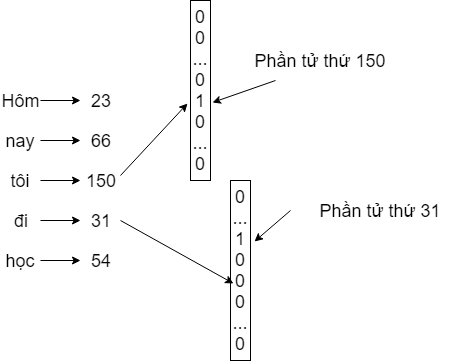
\includegraphics[width=0.8\textwidth]{onehot-representation.png}
	\caption[Minh họa biểu diễn bằng mã hóa one-hot.]{Minh họa biểu diễn bằng mã hóa one-hot. Các từ được đánh số thứ tự trong bộ từ vựng $V$ và chuyển các từ thành các véc-tơ one-hot.}
	\label{fig_onehot-representation}
\end{figure}

Với cách biểu diễn bằng mã hóa one-hot thì ý nghĩa của từ sẽ không bị máy tính hiểu sai như trên tuy nhiên thì các véc-tơ từ này lại không thể hiện được bất kì mối quan hệ nào giữa các từ. Như từ "tôi" và từ "đi" trong hình \ref{fig_onehot-representation} trên, chúng không thể hiện được mối quan hệ về ngữ nghĩa của nó với nhau. Dễ thấy hai véc-tơ này trực giao với nhau nên không có mối quan hệ tương đồng nào. Dù là như thế, nhưng phương pháp mã hóa one-hot này vẫn có được một số các lợi thế. Đó là các từ được biểu diễn dưới dạng các véc-tơ có số chiều bằng nhau. Có rất nhiều thuật toán thao tác trên các dữ liệu mà các điểm dữ liệu có số chiều bằng nhau, do đó thuận lợi hơn cho việc xử lí dữ liệu. Ngoài việc không biểu diễn được các mối quan hệ giữa các từ, mã hóa one-hot còn gặp hạn chế về kích thước của véc-tơ từ. Khi kích thước bộ dữ liệu $V$ lớn như 50000, 100000, 200000, v.v... thì dẫn tới kích thước của các véc-tơ từ cũng lớn theo. Nếu cần xử lí một câu dài hay một đoạn văn thì chi phí tính toán rất lớn, tăng tuyến tính theo số từ cần xử lí là $NV$ ($N$ là số từ).

Vì những hạn chế như vậy, ta cần một cách để giảm thiểu số chiều của những véc-tơ one-hot, đồng thời ta muốn có một cách biểu diễn mà trong đó, các từ có một quan hệ nhất định với nhau như trong ngôn ngữ tự nhiên. Một trong những công trình đầu tiên nghiên cứu về vấn đề này là của giáo sư Geoffrey Hinton \cite{distributedrepHinton}. Trong công trình này, ông đề xuất một biểu diễn của từ gọi là \textit{biểu diễn phân tán} (distributed representation). Biểu diễn phân tán có hai tính chất quan trọng: giảm số chiều không gian và tính tương đồng ngữ nghĩa. Cụ thể, biểu diễn phân tán không còn dùng một phần tử trong véc-tơ để thể hiện một đối tượng nhất định mà các phần tử trong véc-tơ thể hiện một số đặc trưng, tính chất có khả năng phân biệt được các đối tượng. Hình \ref{fig_distributed_representation} minh họa phương pháp biểu diễn phân tán. Các véc-tơ từ sẽ có kích thước nhất định. Mỗi phần tử trong véc-tơ thể hiện một đặc trưng nhất định của một từ. Tất cả các từ được biểu diễn bởi một tập các đặc trưng chung. Các từ sẽ được phân biệt với nhau thông qua các giá trị của các đặc trưng. Phương pháp biểu diễn này có thể biểu diễn được các mối quan hệ giữa các từ với nhau. Ví dụ, để xác định xem từ "Đàn ông" và từ "Phụ nữ" có tính tương đồng về ngữ nghĩa như thế nào: cos\textit{("Đàn ông", "Phụ nữ")}$ = -0.98$. Giá trị này cho thấy rằng từ "Đàn ông" và từ "Phụ nữ" có ý nghĩa trái ngược nhau. Nhìn vào các giá trị đặc trưng của véc-tơ từ của hai từ này, có thể xác định được rằng sự trái ngược về ngữ nghĩa này là về mặt giới tính.

\begin{figure}
	\centering
	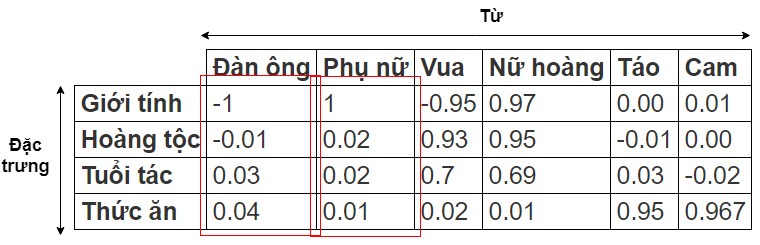
\includegraphics[width=1.0\textwidth]{distributed-representation_1}
	\caption[Minh họa biểu diễn phân tán]{Minh họa biểu diễn phân tán. Để biểu diễn được các từ, phương pháp này sẽ xác định một số đặc trưng, tính chất chung mà dựa vào đó có thể phân biệt được tất cả các từ cần biểu diễn. Mỗi cột là một từ cần được biểu diễn, mỗi dòng là một đặc trưng được dùng để biểu diễn các từ đó.}
	\label{fig_distributed_representation}
\end{figure}

Ví dụ trên đã làm rõ hơn về hai tính chất của biểu diễn phân tán là giảm số chiều không gian và tính tương đồng ngữ nghĩa. Phương pháp này không cần phải sử dụng kích thước véc-tơ lớn tương ứng với số lượng từ mà cần biểu diễn (bộ từ vựng $V$), chỉ cần sử dụng một số lượng đặc trưng nhât định $E$ ($E$ nhỏ hơn rất nhiều so với bộ từ vựng $V$) là có thể biểu diễn được. Những đặc trưng mà véc-tơ từ thể hiện góp phần thể hiện được các phương diện ngữ nghĩa nhất định giữa các từ. Ngoài ra, từ cách biểu diễn các từ bằng các véc-tơ như vậy, biểu diễn phân tán mang lại một số kết quả thú vị khi thực các phép tính số học đối với các véc-tơ từ đó. Sử dụng lại ví dụ được trình bày ở \ref{fig_distributed_representation}, giả sử cần tìm một từ nào mà thỏa mãn mối quan hệ "Đàn ông" $\rightarrow$ "Phụ nữ" $=$ "Vua" $\rightarrow$ $?$. 	Gọi véc-tơ từ cần tìm là $e_k$, có thể biểu diễn mối quan hệ trên lại là: "Đàn ông" $-$ "Phụ nữ" $=$ "Vua" $-$ $e_k$ $\leftrightarrow$ $e_k$ $=$ "Vua" $-$ "Đàn ông" $+$ "Phụ nữ". Thực hiện tính toán, có được véc-tơ từ $e_k = \left[ 1.05, 0.94, 0.69, -0.06\right]^T$. Trong các từ thì $e_k \approx$ "Nữ hoàng" (có khoảng cách tới từ "Nữ hoàng" nhỏ nhất), do đó $e_k =$ "Nữ hoàng". Vậy mối quan hệ tìm được là "Đàn ông" $\rightarrow$ "Phụ nữ" $=$ "Vua" $\rightarrow$ "Nữ hoàng". Đây là tính chất rất hữu ích của biểu diễn phân tán, dựa vào tính chất này, các thuật toán học có thể tận dụng nó để làm tăng độ hiệu quả của mô hình và trực quan hóa các véc-tơ từ bằng cách vẽ đồ thị nhằm có cái nhìn trực quan hơn về các mối quan hệ giữa các từ.

Tuy biểu diễn phân tán có rất nhiều ưu điểm nhưng đi cùng với nó là một nhược điểm lớn và đó cũng là thách thức khó khăn. Làm sao để có thể xây dựng được các véc-tơ từ như vậy? Không thể xây dựng nó bằng cách thủ công như tự định nghĩa các đặc trưng và gán các giá trị cho từng từ trong bộ từ vựng được bởi vì công sức làm việc đó là rất lớn khi kích thước bộ từ vựng lớn lên. Các đặc trưng tự định nghĩa cũng rất khó thể hiện chính xác hoàn toàn được những ngữ nghĩa của các từ theo mong đợi. Do đó, các thuật toán, mô hình học biểu diễn phân tán một cách tự động được ra đời. Các thuật toán, mô hình như thế được gọi chung là \textit{word embedding} (tạm dịch là \textit{phép nhúng từ}).

Word embedding được đề xuất bởi giáo sư Yoshua Bengio và cộng sự vào năm 2003 \cite{bengioLM2003} khi họ đã huấn luyện một mô hình ngôn ngữ nơ-ron đồng thời với các tham số của mô hình. Tuy nhiên công trình này vẫn chưa thực sự thành công, cho tới năm 2008, Collobert và Weston \cite{wordembeddingCollobert2008} đã đề xuất một kiến trúc mạng nơ-ron sâu tổng quát cho bài toán này.

Để hiểu được tại sao word embedding là một phương pháp biểu diễn từ mạnh mẽ, hãy tìm hiểu cách hoạt động của nó. Giả sử đầu vào của một mô hình word embedding là một chuỗi gồm $T$ véc-tơ one-hot $(w_1,w_2,...,w_{T})$. Để tạo thành véc-tơ embedding, những véc-tơ one-hot sẽ được nhân với một ma trận của phép biến đổi tuyến tính $P$. Các véc-tơ one-hot sẽ trở thành những véc-tơ \textit{liên tục} $(x_1, x_2,...,x_{T})$ sao cho,

\begin{equation} \label{wordembeddingmatrix}
x_j = Pw_j
\end{equation}

Lưu ý rằng phép nhân ma trận này không được thực hiện như phép nhân ma trận thông thường. Bởi vì $w_j$ chỉ có một phần tử có giá trị $1$ (phần tử thứ $j$) và tất cả những phần tử còn lại mang giá trị $0$. Cho nên phép nhân này tương đương với lấy cột thứ $j$ của $P$. Phép truy xuất ma trận thì nhanh hơn rất nhiều lần so với phép nhân ma trận nên phép toán \ref{wordembeddingmatrix} sẽ không tốn nhiều chi phí. Ban đầu ma trận $P$ sẽ được khởi tạo ngẫu nhiên, trong học sâu, tùy vào từng bài toán mà những ma trận này sẽ được học bằng thuật toán lan truyền ngược (backpropagation).

Word embedding không chỉ giải quyết vấn đề của véc-tơ one-hot, mà nó còn là một phương pháp mạnh mẽ cho bài toán mô hình hóa ngôn ngữ. Ở phần mô hình ngôn ngữ, chúng tôi có nhắc đến việc mô hình \textit{n}-gram xem những từ trong tập ngữ liệu là rời rạc. Nếu trong tập ngữ liệu không có từ "bath room" mà chỉ có "bed room" thì mô hình \textit{n}-gram sẽ gán xác suất $0$ cho "bath room", mặc dù hai \textit{n}-gram này có mối liên quan khá lớn với nhau. Điều này làm cho tính tổng quát hóa của mô hình \textit{n}-gram không cao. Khác với mô hình \textit{n}-gram, mô hình word embedding có khả năng tổng quát hóa cao với những \textit{n}-gram chưa nhìn thấy. Lấy ví dụ một mô hình ngôn ngữ bằng mạng nơ-ron truyền thẳng đơn giản gồm hai hàm thành phần $f$ và $g$. Hàm $f$ ánh xạ một chuỗi $k$ từ trước đó sang một véc-tơ liên tục. Véc-tơ liên tục $h$ được coi là véc-tơ ngữ cảnh với từ cần dự đoán.

\begin{equation} \label{contextvectorfnnlm1}
f: \{0,1\}^{|V| \times k} \rightarrow \mathbb{R}^{d}
\end{equation}
với $d$ là kích thước của word embedding mà ta chọn.

Tiếp theo, hàm $g$ thực hiện ánh xạ véc-tơ ngữ cảnh $h$ sang một véc-tơ phân bố xác suất nhằm dự đoán từ tiếp theo trong chuỗi.
\begin{equation} \label{contextvectorfnnlm2}
g(h) = \softmax \left(Uh \right)
\end{equation}
để cho đơn giản, chúng tôi đã bỏ đi véc-tơ bias của phép biến đổi.

\begin{figure}
	\centering
	\includegraphics[width=0.6\textwidth]{embeddingmapping}
	\caption[Minh họa quá trình biến đổi của phép nhân ma trận]{Minh họa quá trình biến đổi của phép nhân ma trận.}
	\label{fig_embedding_mapping}
\end{figure}

Hình \ref{fig_embedding_mapping} miêu tả phép nhân giữa ma trận $U$ và véc-tơ $h$. Nhận thấy rằng thành phần thứ $i$ của véc-tơ kết quả chính là $h^tu_i$. Điều này có nghĩa là xác suất để từ thứ $i$ trong bộ từ vựng là từ tiếp theo xuất hiện tỷ lệ thuận với kết quả $h^tu_i$.

Nếu có hai chuỗi ngữ cảnh được theo sau bởi cùng một tập các từ thì hai véc-tơ ngữ cảnh $h_1$ và $h_2$ của chúng phải gần giống nhau. Vì khi nhân hai véc-tơ này với cùng ma trận $U$, mô hình đều cần những từ theo sau phải có xác suất lớn trong véc-tơ dự đoán. Điều này có nghĩa là nếu một mô hình ngôn ngữ được huấn luyện tốt, nó sẽ phải chiếu những \textit{n}-gram được theo sau bởi cùng một tập từ thành những véc-tơ gần nhau trong không gian liên tục.

Xét một ví dụ về word embedding, trong đó ta quy định bậc của giả định markov là 1, tức là từ tiếp theo chỉ phụ thuộc vào từ ngay trước nó. Những \textit{n}-gram được \textbf{in đậm} là những \textit{n}-gram cần quan tâm:
\begin{itemize}
	\item[1.] There are \textbf{ten teams} participating in the competition.
	\item[2.] \textbf{four teams} have passed the first round.
	\item[3.] \textbf{four groups} are playing in the field.
\end{itemize}

Với những phân tích trước đó, hai từ \textbf{ten} và \textbf{four} sẽ có biểu diễn gần giống nhau vì chúng đều dự đoán từ \textbf{teams}. Hơn thế nữa, các véc-tơ từ tương ứng với \textbf{teams} $u_{teams}$ và \textbf{groups} $u_{groups}$ trong ma trận $U$ cũng sẽ gần giống nhau. Bởi vì nếu không xác suất của \textbf{teams} khi biết \textbf{four} $p(teams|four) \propto u_{teams}h_{four}$ và xác suất của \textbf{groups} khi biết \textbf{four} $p(groups|four) \propto u_{groups}h_{four}$ sẽ khác nhau mặc dù chúng có cùng xác suất trong tập ngữ liệu (câu thứ 2 và 3 trong tập dữ liệu gồm 3 câu phía trên).

Giả sử tập ngữ liệu gồm 3 câu này được sử dụng để huấn luyện một mô hình ngôn ngữ. Xét một bi-gram chưa từng xuất hiện trong tập ngữ liệu là \textbf{ten groups}. Ta biết rằng, mô hình ngôn ngữ gán cho \textbf{ten} một véc-tơ $h_{ten}$ gần với véc-tơ của \textbf{four} $h_{four}$. Sau đó từ véc-tơ ngữ cảnh của $h_{ten}$, mô hình sẽ phải gán cho xác suất $p(group|ten)$ một giá trị lớn, vì $h_{ten} \approx h_{four}$ mà $h_{four}$ và $u_{group}$ đã được gióng hàng tốt với nhau. Rõ ràng là mặc dù bi-gram \textbf{ten groups} chưa từng xuất hiện trong tập ngữ vựng, nhưng mô hình vẫn gán cho nó một xác suất hợp lý. 

Có thể tóm gọn lại nguyên lý của word embedding là với những từ trong cùng một ngữ cảnh (ngữ cảnh là những từ xung quanh nó) sẽ có véc-tơ embedding giống nhau, và những ngữ cảnh giống nhau cũng sẽ có các véc-tơ tương tự nhau trong không gian ngữ cảnh. Nguyên lý này rất đẹp và có ý nghĩa đối với những bài toán cần dùng đến tính chất ngữ nghĩa của các từ và câu, như trong bài toán dịch máy.

Hiện nay, có hai cách chính để học word embedding.
\begin{itemize}
	\item Học theo chiến lược học không giám sát: sử dụng các thuật toán học đặc biệt để học biểu diễn từ dựa trên một tập dữ liệu. Thường là những tập dữ liệu thu thập được từ các nguồn khác nhau về mà chưa có được xử lí, đánh nhãn để giải quyết cho một bài toán cụ thể nào. Các tập dữ liệu này thường là dùng để huấn luyện cho mô hình ngôn ngữ.
	\item Học theo chiến lược có giám sát: các véc-tơ biểu diễn từ là một phần của một mô hình học có giám sát, cụ thể là các tham số trong mô hình. Mô hình sẽ học đồng thời cách giải quyết bài toán và các véc-tơ biểu diễn từ. Tùy thuộc vào bài toán mà mô hình này giải quyết như Dịch máy, Phân tích ý kiến của người dùng, các véc-tơ biểu diễn từ học được sẽ phù hợp duy nhất cho bài toán đó.
\end{itemize}

Hiện nay học theo chiến lược học không giám sát đang có được những kết quả ấn tượng. Cách học này giúp word embedding học được thường tốt hơn do tập dữ liệu không cần nhãn, vì thế tập dữ liệu dành cho việc học word embedding là rất lớn (có thể lên tới 1 tỉ từ) do dễ thu thập. Hơn nữa, word embedding học được còn có khả năng tổng quát hóa tốt (biểu diễn từ học được tốt trong nhiều ngữ cảnh). Đại diện cho cách học này là gồm Word2Vec \cite{word2vec2013} (sử dụng một mạng nơ-ron và ý tưởng đơn giản để học) và GloVe \cite{glove2014} (sử dụng thống kê tần số của các từ để học). Đây là hai word embedding mà được mọi người tin tưởng và sử dụng rộng rãi để giải quyết các bài toán khác nhau.

Học theo chiến lược có giám sát thì ít phổ biến hơn bởi vì word embedding học được theo cách này thì chỉ có hữu dụng với bài toán mà mô hình đang giải quyết. Nếu như mô hình đang giải quyết bài toán Dịch máy thì word embedding sẽ tâp trung vào biểu diễn các từ sao cho phù hợp nhất với bài toán Dịch máy và không thể mang word embedding này để giải quyết bài toán khác. Trong khóa luận này, cách học word embedding theo học có giám sát được sử dụng để biểu diễn các từ trong câu đầu vào và câu đầu ra. Một tầng Embedding được sử dụng để thực hiện mã hóa các từ đầu vào thành các véc-tơ biểu diễn phân tán với kích thước véc-tơ được cho trước. Tầng Embedding này đơn giản là một mạng nơ-ron truyền thẳng mà không có tầng ẩn với đầu vào véc-tơ one-hot và đầu ra là véc-tơ biểu diễn phân tán.

\begin{figure}
	\centering
	\includegraphics[width=0.9\textwidth]{Embedding_layer.png}
	\caption[Minh họa tầng Embedding.]{Minh họa tầng Embedding. Tầng Embedding này đơn giản là một mạng nơ-ron truyền thẳng mà không có tầng ẩn với đầu vào véc-tơ one-hot và đầu ra là véc-tơ biểu diễn phân tán. Các trọng số của mạng $E$ chính là word embedding học được. Mỗi một cột thứ $i$ trong ma trận $E$ là một véc-tơ biểu diễn phân tán cho từ có thứ $i$ trong bộ từ vựng.}
	\label{fig_embedding_layer}
\end{figure}

\section{Mạng nơ-ron hồi quy (Recurrent neural network)} \label{rnnsection}

Trong tự nhiên, dữ liệu không phải lúc nào cũng được sinh ra một cách ngẫu nhiên. Trong một số trường hợp, chúng được sinh ra theo một thứ tự. Xét trong dữ liệu văn bản, ví dụ ta cần điền vào chỗ trống cho câu sau \textit{"Paris là thủ đô của nước \_\_"}. Dễ biết được rằng chỉ có duy nhất một từ phù hợp cho chỗ trống này, đó là \textit{"Pháp"}. Điều này có nghĩa là mỗi từ trong một câu không được tạo ra ngẫu nhiên mà nó được tạo ra dựa trên một liên hệ với những từ đứng trước nó. Các loại dữ liệu khác như những khung hình trong một bộ phim hoặc các đoạn âm thanh trong một bản nhạc cũng có tính chất tương tự. Những loại dữ liệu mang thứ tự này được gọi chung là dữ liệu chuỗi (sequential data).

Trong quá khứ, một số mô hình xử lý dữ liệu chuỗi bằng cách giả định rằng đầu vào hiện tại có liên hệ với một số lượng xác định đầu vào trước đó, nhiều mô hình tạo ra một cửa sổ trượt để nối mỗi đầu vào hiện tại với một số lượng đầu vào trước đó nhằm tạo ra sự mô phỏng về tính phụ thuộc. Cách tiếp cận này đã được sử dụng cho mô hình \textit{Deep belief network} trong xử lý tiếng nói \cite{massetal2012}. Nhược điểm của những cách làm này là ta phải xác định trước kích thước của cửa sổ. Một mô hình với kích thước cửa sổ với chiều dài bằng 6 không thể nào quyết định được từ tiếp theo trong câu \textit{"Hổ là loài động vật ăn \_\_"} sẽ là \textit{"thịt"} hay \textit{"cỏ"}. Trong ví dụ này, từ tiếp theo của câu phụ thuộc mật thiết vào từ \textit{"Hổ"} cách nó đúng 6 từ. Trên thực tế, có rất nhiều câu đòi hỏi sự phụ thuộc với nhiều từ xa hơn trước đó. Ta gọi những sự phụ thuộc kiểu như vậy là những \textit{phụ thuộc dài hạn} (long term dependency). 

\textit{Mạng nơ-ron hồi quy} (recurrent neural network) \cite{elman1990} gọi tắt là \textit{RNN} là một nhánh của nạng nơ-ron nhân tạo được thiết kế đặc biệt cho việc mô hình hóa dữ liệu chuỗi. Khác với những mô hình đã đề cập giả định sự phụ thuộc chỉ xảy ra trong một vùng có chiều dài cố định. RNN, trên lý thuyết, có khả năng nắm bắt được các phụ thuộc dài hạn với chiều dài bất kỳ. Để làm được điều đó, trong quá trình học, RNN lưu giữ những thông tin cần thiết cho các phụ thuộc dài hạn bằng một véc-tơ được gọi là \textit{trạng thái ẩn}.

Xét một chuỗi đầu vào $x={x_1,x_2,...,x_n}$. Gọi $h_t$ là trạng thái ẩn tại \textit{bước thời gian} (timestep) $t$, là lúc một mẫu dữ liệu $x_t$ được đưa vào RNN để xử lý. Trạng thái ẩn $h_t$ sẽ được tính toán dựa trên mẫu dữ liệu hiện tại $x_t$ và trạng thái ẩn trước đó $h_{t-1}$. Có thể thể hiện $h_t$ như một hàm hồi quy với tham số là đầu vào hiện tại và chính nó ở thời điểm trước đó:
\begin{equation} \label{basicRnnEquation}
h_t = f \left(h_{t-1}, x_t \right)
\end{equation}
trong đó hàm $f$ là một ánh xạ phi tuyến. Có thể hình dung $h_t$ như một đại diện cho những đầu vào mà nó đã xử lý từ thời điểm ban đầu cho đến thời điểm $t$. Nói một cách khác, RNN sử dụng trạng thái ẩn như một dạng bộ nhớ để lưu giữ thông tin từ một chuỗi. Hình \ref{fig_rnn_loop} thể hiện định nghĩa hồi quy của RNN.

\begin{figure}
	\centering
	\includegraphics[width=0.25\textwidth]{rnn_loop}
	\caption[Mô hình RNN với kết nối vòng]{Mô hình RNN đơn giản với kết nối vòng, \textbf{$h$} được xem như bộ nhớ được luân chuyển trong RNN. Ô vuông với ký hiệu "A" trong hình được gọi là một tế bào RNN. Chú ý rằng đường nét đứt ở đầu ra thể hiện rằng tại một thời điểm $t$, RNN có thể có hoặc không có một đầu ra.}
	\label{fig_rnn_loop}
\end{figure}
Thông thường, hàm $f$ là một hàm phi tuyến như hàm \textbf{sigmoid} hay hàm \textbf{tanh}. Xét một RNN với công thức cụ thể như sau:
\begin{equation} \label{rnnWithTanh}
h_t = \phi \left(W_{xh} x_t + W_{hh}h_{t-1} + b_h \right)
\end{equation}
Trong đó:
\begin{itemize}
	\item[•] $\phi$ là một hàm kích hoạt (ví dụ: sigmoid, tanh hay ReLU).
	\item[•] $h_{t} \in \mathbb{R}^{D_h}$ là trạng thái ẩn tại bước thời gian hiện tại có chiều dài $D_h$.
	\item[•] $x_t \in \mathbb{R}^{D_x}$ là véc-tơ đầu vào hiện tại có chiều dài $D_x$.
	\item[•] $h_{t-1} \in \mathbb{R}^{D_h}$ là trạng thái ẩn tại bước thời gian trước đó.
	\item[•] $W_{xh} \in \mathbb{R}^{D_x \times D_h}, W_{hh} \in \mathbb{R}^{D_h \times D_h}$ và $b_h \in \mathbb{R}^{D_h}$ lần lượt là hai ma trận trọng số và véc-tơ bias.
\end{itemize}

Ma trận $W_{xh}$ là làm nhiệm vụ kết nối giữa đầu vào và trạng thái ẩn, $W_{hh}$ kết nối trạng thái ẩn với chính nó trong các bước thời gian liền kề. Véc-tơ $b_h$ dùng để điều chỉnh giá trị của $h_t$. Tại thời điểm bắt đầu, trạng thái ẩn $h_0$ có thể được khởi tạo bằng 0 hoặc là một véc-tơ chứa tri thức có sẵn như trường hợp của bộ giải mã như chúng tôi đã đề cập trong chương 1.

Tại mỗi bước thời gian $t$, tùy vào mục tiêu cụ thể của quá trình học mà RNN có thể có thêm một đầu ra $y_t$. Trong ngữ cảnh bài toán dịch máy nơ-ron, đầu ra của RNN trong quá trình giải mã chính là một từ trong ngôn ngữ đích hay nói chung là một đầu ra dạng rời rạc. Với mục tiêu đó, đầu ra dự đoán của RNN $\hat{y}_t$ sẽ có dạng là một phần phối xác suất trên tập các các lớp ở đầu ra. Phân phối này nhằm dự đoán vị trí xuất hiện của $\hat{y}_t$.
%\begin{equation} \label{rnnOuputSoftmax}
%	s_t = W_{hy}h_t + b_y
%\end{equation} 
\begin{equation} \label{rnnOuputSoftmaxDistribution}
\hat{y}_t = \softmax(W_{hy}h_t + b_y)
\end{equation}
Trong đó:
\begin{itemize}
	\item[•] $\softmax$ là một hàm kích hoạt với $\softmax(v) = \frac{e^{v_j}}{\sum_{k=1}^{K}e^{v_k}}$, $j = 1,...,K$. $K$ là độ dài của véc-tơ $v$.
	\item[•] $h_{t} \in \mathbb{R}^{D_h}$ là trạng thái ẩn tại bước thời gian hiện tại.
	\item[•] $W_{hy} \in \mathbb{R}^{L \times D_h}$ và $b_y \in \mathbb{R}^L$ lần lượt là hai ma trận trọng số và véc-tơ bias. $L$ là số lượng lớp cần phân biệt ở đầu ra.
\end{itemize}

Trong công thức trên, hàm $\softmax$ đóng vai trò là một hàm chuẩn hóa để $\hat{y}_t$ thể hiện một phân phối xác suất trên các lớp ở đầu ra. Ma trận $W_{hy}$ kết nối đầu ra với trạng thái ẩn, $b_y$ dùng để điều chỉnh giá trị của kết quả tính toán trước khi đưa qua hàm $\softmax$.

\begin{figure}
	\centering
	\includegraphics[width=0.85\textwidth]{rnn_unrolled}
	\caption[Mô hình RNN dạng dàn trải]{Mô hình RNN được dàn trải (unrolled), ví dụ trong 4 bước thời gian.}
	\label{fig_rnn_unrolled}
\end{figure}

Để ý rằng các ma trận trọng số $W_{xh}$, $W_{hh}$, $W_{hy}$ và các véc-tơ bias $b_h$, $b_y$ là các tham số học của mô hình và chúng là duy nhất. Có nghĩa là khi những tham số này được học, bất kỳ một đầu vào nào cũng đều sử dụng chung một bộ tham số. Điều này chính là sự chia sẻ tham số (parameters sharing) trong mạng nơ-ron hồi quy. Chia sẻ tham số khiến cho mô hình học dễ dàng hơn, nó giúp cho RNN có thể xử lý chuỗi đầu vào với độ dài bất kỳ mà không làm tăng độ phức tạp của mô hình. Quan trọng hơn, nó giúp ích cho việc tổng quát hóa. Đây chính là điểm đặc biệt của RNN so với mạng nơ-ron truyền thẳng (feedforward neural network).

Với một số lượng hữu hạn các bước thời gian, mô hình RNN trên hình \ref{fig_rnn_loop} có thể được dàn trải ra (unrolled). Dạng dàn trải này được miêu tả trực quan như trên hình \ref{fig_rnn_unrolled}. Với cách thể hiện này, RNN có thể được hiểu như là một mạng nơ-ron sâu với mỗi bước thời gian là một mạng nơ-ron một tầng ẩn và các tham số học được chia sẻ giữa các mạng nơ-ron đó. Dạng dàn trải cũng thể hiện rằng RNN có thể được huấn luyện qua nhiều bước thời gian bằng thuật toán lan truyền ngược (backpropagation). Thuật toán này được gọi là Backpropagation through time (BPTT) \cite{werbos1990}. Thực chất đây là chỉ thuật toán “Backpropagation” khi áp dụng cho RNN dưới dạng dàn trải để tính gradient cho các tham số ở từng bước thời gian. Hầu hết cả các mạng nơ-ron hồi quy phổ biến ngày nay đều áp dụng thuật toán này vì tính đơn giản và hiệu quả của nó.

\subsection{Huấn luyện mạng nơ-ron hồi quy}

Xét một chuỗi đầu vào $x={x_1,x_2,...,x_n}$ với đầu ra tương ứng $y={y_1,y_2,...,y_n}$. Trong quá trình lan truyền tiến, tại mỗi bước thời gian $t$ ứng mẫu dữ liệu $(x_t, y_t)$, công thức tính toán đầu ra dự đoán có dạng:
\begin{equation} \label{rnnForwardProp1}
h_t = \phi \left(W_{xh} x_t + W_{hh}h_{t-1} + b_h \right) 
\end{equation}
\begin{equation} \label{rnnForwardProp2}
s_t = W_{hy} h_t + b_y 
\end{equation}
\begin{equation} \label{rnnForwardProp3}
\hat{y}_t = \softmax (s_t) 
\end{equation}
Như trong các bài toán học có giám sát khác, ta cần định nghĩa hàm độ lỗi giữa đầu ra dự đoán $\hat{y}_t$ và đầu ra thật sự $y_t$. Với $L$ là số lượng lớp của $y$, lúc này có thể thấy $\hat{y}_t$ là một véc-tơ phân phối xác suất có độ dài $L$. Để so sánh với $\hat{y}_t$, $y_t$ được chuẩn hóa thành một véc-tơ dạng one hot có nghĩa là một véc-tơ với độ dài $V$ có giá trị bằng 0 trừ vị trí ứng với lớp của $y_t$ có giá trị 1. Như vậy để so sánh hai phân phối xác suất $y$ và $\hat{y}$ hàm độ lỗi \textit{negative log-likelihood} hay còn gọi là \textit{cross entropy} sẽ được sử dụng, gọi $L_t$ là độ lỗi tại một bước thời gian $t$:
\begin{equation} \label{errorOfAnExample}
L_t = -y_t^{T} \log(\hat{y}_t)
\end{equation}

Gọi $\theta$ là một tham số của mô hình, biết rằng $\theta$ được chia sẻ trong quá trình học, tức là ở mọi bước thời gian, chúng đều có giá trị bằng nhau:
\begin{equation} \label{weightSharing1}
\theta_t = \theta_k
\end{equation}
Với $t$, $k$ là những bước thời gian ($t \ne k$). Tại thời điểm bắt đầu với $t=k=0$ mọi $\theta_i$ đều có giá trị bằng nhau nên trong quá trình học, gradient của chúng cũng cần bằng nhau:
\begin{equation} \label{weightSharing2}
\frac{\partial L}{\partial \theta_t} = \frac{\partial L}{\partial \theta_k}
\end{equation}
Với $L$ là độ lỗi tổng hợp tại của tất cả các bước thời gian. Như vậy để $\theta_t = \theta_k, \forall t;k$, ta chỉ đơn giản xem $L$ là tổng độ lỗi ở tất cả các bước thời gian. Với cách làm này, tham số luôn bằng nhau sau mỗi lần cập nhật.
\begin{equation} \label{errorOfAll}
L = \sum_{t}L_t = - \sum_{t} y_t^{T} \log(\hat{y}_t) 
\end{equation}

% TODO: tai sao su dung mini batch
Mục tiêu của việc học là cực tiểu hóa độ lỗi tổng hợp $L$. Thuật toán backpropagation với \textit{gradient descent} sẽ được áp dụng để huấn luyện RNN. Trên thực tế, người ta sẽ sử dụng một phiên bản của gradient descent là mini-batch gradient descent cho việc huấn luyện. Tập dữ liệu ban đầu sẽ được chia thành nhiều mini-batch, mỗi mini-batch là một tập con với số lượng khoảng vài chục đến vài trăm mẫu thuộc tập dữ liệu ban đầu. Với mỗi lần duyệt (iteration), việc tính toán gradient để cập nhật các tham số học của mô hình được thực hiện lần lượt trên tất cả các mini-batch này.

Mô hình cần tìm bộ tham số $\theta \in \left\{W_{hy},W_{hh},W_{xh},b_y,b_h \right \}$ sao cho cực tiểu hóa hàm độ lỗi $L$. Theo thuật toán gradient descent, bộ tham số được cập nhật theo công thức:
\begin{equation} \label{gradientDescentWithTheta}
\theta \leftarrow \theta - \eta \nabla_{\theta} L
\end{equation}

% TODO: Bo sung cho nay
Ở đây, $\nabla_{\theta} L$ là gradient của hàm độ lỗi ứng với tham số $\theta$. $\eta$ được gọi là hệ số học (learning rate) là một siêu tham số quyết định rằng $\theta$ sẽ thay đổi nhiều bao nhiêu theo giá trị gradient tính được. Trong phần dưới đây, chúng tôi sẽ trình bày việc tính toán gradient của hàm độ lỗi theo bộ tham số học $\theta \in \left\{W_{hy},W_{hh},W_{xh},b_y,b_h \right \}$.

Với $s_t = W_{hy} h_t + b_y$ và $\hat{y}_t = \softmax(s_t)$, sử dụng chain rule trong tính đạo hàm ta được:
%\nabla_{\theta} L_t = \frac{\partial h_t}{\partial \theta} \frac{\partial s_t}{\partial h_t} \frac{\partial \hat{y}_t}{\partial s_t} \frac{\partial L_t}{\partial \hat{y}_t} = \frac{\partial h_t}{\partial \theta}  \frac{\partial s_t}{\partial h_t} \frac{\partial L_t}{\partial s_t}

\begin{equation} \label{gradientCalculating1}
\nabla_{\theta} L_t = \frac{\partial L_t}{\partial \hat{y}_t} \frac{\partial \hat{y}_t}{\partial s_t} \frac{\partial s_t}{\partial h_t} \frac{\partial h_t}{\partial \theta}  = \frac{\partial L_t}{\partial s_t} \frac{\partial s_t}{\partial h_t} \frac{\partial h_t}{\partial \theta}
\end{equation}

Và có:
\begin{equation} \label{gradientCalculating2}
\nabla_{s_t}L_t = \frac{\partial L_t}{\partial s_t} = \hat{y}_t - y
\end{equation}

Dễ dàng tính được:
\begin{equation} \label{gradientCalculating3}
\frac{\partial s_t}{\partial h_t} = W_{hy}^T
\end{equation}

Đến đây, chỉ cần tìm $\frac{\partial h_t}{\partial \theta}$ với $\theta \in \left\{W_{hy},W_{hh},W_{xh},b_y,b_h \right \}$. Có thể chia các tham số thành hai nhóm. Nhóm đầu tiên là các tham số liên quan đến quá trình tính toán đầu ra, bao gồm $\theta^{(1)} \in \{W_{hy}, b_y\}$. Những tham số này không tham gia vào hàm hồi quy $h_t$ cho nên gradient ứng với chúng được tính một cách dễ dàng:

\begin{equation} \label{gradientCalculating4}
\nabla_{W_{hy}}L_t = \frac{\partial L_t}{\partial s_t} \frac{\partial s_t}{\partial W_{hy}}  =  (\hat{y}_t - y) h_t^T
\end{equation}
\begin{equation} \label{gradientCalculating5}
\nabla_{b_{y}}L_t = \frac{\partial L_t}{\partial s_t} \frac{\partial s_t}{\partial b_{y}}  =  \hat{y}_t - y
\end{equation}

Nhóm thứ hai gồm những tham số tham gia vào quá trình hồi quy, bao gồm $\theta^{(2)} \in \{W_{hh},W_{xh},b_h \}$. Để tính được gradient ứng với $\theta^{(2)}$, cần tính được $\frac{\partial h_t}{\partial \theta^{(2)} }$

Vì $h_t$ là một hàm hồi quy được xây dựng dựa trên $\theta^{(2)}$ và $h_{t-1}$ nên gradient cuả $h_t$ tương ứng với $\theta^{(2)}$ được tính dựa trên quy tắc \textit{total derivative}. Quy tắc này nói rằng nếu $f(x,y)$ với $x, y \in \mathbb{R}^M$, giả sử $x,y$ là những hàm số của $r$ sao cho $x = x(r); y = y(r)$ thì ta có:
\begin{equation} \label{gradientWRTSt6}
\frac{\partial{f}}{\partial{r}} = \frac{\partial f}{\partial x}\frac{\partial x }{\partial r} + \frac{\partial f }{\partial y }\frac{\partial y }{\partial r }
\end{equation}

Áp dụng vào trường hợp của $\frac{\partial h_t}{\partial \theta^{(2)} }$ ta được:
\begin{equation} \label{gradientWRTSt7}
\frac{\partial h_t}{ \partial \theta^{(2)}} = \frac{\partial h_t}{ \partial \theta^{(2)}} + \frac{\partial h_t }{\partial h_{t-1} } \frac{\partial h_{t-1}}{ \partial \theta^{(2)}}
\end{equation}

Tuy nhiên, ta có thể khai triển công thức trên một lần nữa với cách làm tương tự cho $\frac{\partial h_{t-1}}{\partial \theta^{(2)} }$:
\begin{equation} \label{gradientWRTSt8}
\frac{\partial h_t}{\partial \theta^{(2)}} = \frac{\partial h_t}{\partial \theta^{(2)}} + \frac{\partial h_t }{\partial h_{t-1}} \frac{\partial h_{t-1}}{\partial \theta^{(2)}} + \frac{\partial h_t}{\partial h_{t-1}} \frac{\partial h_{t-1}}{\partial h_{t-2}} \frac{\partial h_{t-2}}{\partial \theta^{(2)}}
\end{equation}

Khai triển trên sẽ kéo dài cho đến khi gặp $\frac{\partial h_0}{\partial \theta^{(2)}}$. Và để ý rằng:
\begin{equation} \label{gradientWRTSt9}
\frac{\partial h_t}{\partial h_{t-1}} \frac{\partial h_{t-1}}{\partial h_{t-2}} \frac{\partial h_{t-2}}{\partial \theta^{(2)}} = \frac{\partial h_t}{\partial h_{t-2}}\frac{\partial h_{t-2}}{\partial \theta^{(2)}}
\end{equation}
\begin{equation} \label{gradientWRTSt10}
\frac{\partial h_{t}}{\partial \theta^{(2)}} = \frac{\partial h_{t}}{\partial h_t} \frac{\partial h_t}{\partial \theta^{(2)}}
\end{equation}

Với cách khai triển như vậy, công thức tổng quát cho $\frac{\partial h_t}{\partial \theta^{(2)}}$ sẽ là:
\begin{equation} \label{gradientWRTSt11}
\frac{\partial h_t}{\partial \theta^{(2)}} = \sum_{r=0}^{t} \frac{\partial h_{t}}{\partial h_r} \frac{\partial^{\dagger} h_r}{\partial \theta^{(2)}}
\end{equation}
trong đó $\frac{\partial^{\dagger} h_r}{\partial \theta^{(2)}}$ là đạo hàm "lập tức", có nghĩa là khi lấy đạo hàm $h_r$ theo $\theta^{(2)}$, $h_{r-1}$ được coi là hằng số.

Lần lượt thay thế $\theta^{(2)}$ bằng $W_{hh}, W_{xh}, b_h$ gradient ứng với từng tham số là:
\begin{equation} \label{gradientWRTSt12}
\nabla_{W_{hh}}L_t = \frac{\partial L_t}{\partial s_t} \frac{\partial s_t}{\partial h_t} \frac{\partial h_t}{\partial W_{hh}}  =  (\hat{y}_t - y) W_{hy}^T \sum_{r=0}^{t} \frac{\partial h_{t}}{\partial h_r} \frac{\partial h_r}{\partial W_{hh}}
\end{equation}
\begin{equation} \label{gradientWRTSt13}
\nabla_{W_{xh}}L_t = \frac{\partial L_t}{\partial s_t} \frac{\partial s_t}{\partial h_t} \frac{\partial h_t}{\partial W_{xh}}  =  (\hat{y}_t - y) W_{hy}^T \sum_{r=0}^{t} \frac{\partial h_{t}}{\partial h_r} \frac{\partial h_r}{\partial W_{xh}}
\end{equation}
\begin{equation} \label{gradientWRTSt14}
\nabla_{b_h}L_t = \frac{\partial L_t}{\partial s_t} \frac{\partial s_t}{\partial h_t} \frac{\partial h_t}{\partial b_h}  =  (\hat{y}_t - y) W_{hy}^T \sum_{r=0}^{t} \frac{\partial h_{t}}{\partial h_r} \frac{\partial h_r}{\partial b_h}
\end{equation}

Để tính $\frac{\partial h_t}{\partial h_r}$ ta áp dụng chain rule từ bước thời gian thứ $t$ đến $r$
\begin{equation} \label{gradientWRTSt15}
\frac{\partial h_t}{\partial h_r} = \prod_{i=r}^{t} \frac{\partial h_{i}}{\partial h_{i-1}}
\end{equation}
với $h_{i+1},h_i \in \mathbb{R}^n$ nên $\frac{\partial h_{i}}{\partial h_{i-1}}$ là một ma trận "Jacobian"

\begin{equation} \label{gradientWRTSt16}
\begin{split}
\frac{\partial h_{i}}{\partial h_{i-1}} &= \left[ \frac{h_{i}}{h_{i-1,1}}, ..., \frac{h_{i}}{h_{i-1,n}} \right] \\
&= \begin{bmatrix}
\frac{h_{i, 1}}{h_{i-1,1}} & \cdots & \frac{h_{i,1}}{h_{i-1,n}}\\
\vdots & \ddots & \vdots\\
\end{bmatrix} \\
&= W_{hh}^T \diag \left( \phi'(h_i) \right)
\end{split} 
\end{equation}

Như vậy, ta có gradient của các tham số qua tất cả các bước thời gian sẽ là:

\begin{align}
\nabla_{b_{y}}L &= \sum_{t} \hat{y}_t - y \\ \label{updateParams2} 
\nabla_{b_h}L &= \sum_{t} \sum_{r=0}^{t} (\hat{y}_t - y) W_{hy}^T \frac{\partial h_{t}}{\partial h_r} \frac{\partial h_r}{\partial b_h} \\ \label{updateParams3}
\nabla_{W_{hy}}L &= \sum_{t} (\hat{y}_t - y) h_t^T \\ \label{updateParams4}
\nabla_{W_{hh}}L &= \sum_{t} \sum_{r=0}^{t}  (\hat{y}_t - y) W_{hy}^T \frac{\partial h_{t}}{\partial h_r} \frac{\partial h_r}{\partial W_{hh}} \\ \label{updateParams5}
\nabla_{W_{xh}}L_t &= \sum_{t} \sum_{r=0}^{t} (\hat{y}_t - y) W_{hy}^T \frac{\partial h_{t}}{\partial h_r} \frac{\partial h_r}{\partial W_{xh}} \\ \label{updateParams6} \nonumber
\end{align}

\subsection{Thách thức trong việc học các phụ thuộc dài hạn}

Mặc dù việc tính toán các gradient trong RNN là đơn giản, tuy nhiên việc huấn luyện để tạo ra một RNN hoạt động tốt là vô cùng khó. Khó khăn đó đến từ hai vấn đề: một là việc \textit{mất mát thông tin} (information morphing) và hai là \textit{sự biến mất và sự bùng nổ gradient} (vanishing and exploding gradient).

Đầu tiên, về sự mất mát thông tin: nếu thông tin liên tục bị mất mát, rất khó để khai thác thông tin trong quá khứ khi ta cần nó. Giả sử mô hình cần thông tin về động từ của một câu để phân biệt một câu đó là tích cực hay tiêu cực, sau khi đọc qua toàn bộ câu bằng một RNN, ta tiến hành phân lớp dựa trên trạng thái ẩn cuối cùng của RNN. Tuy nhiên, trong RNN, thông tin sẽ bị mất mát đi khi được lan truyền qua nhiều bước thời gian do hai lý do: 
\begin{itemize}
	\item[•] Trạng thái ẩn của RNN là một véc-tơ có kích thước cố định, trong quá trình lan truyền tiến, thông tin được ghi liên tục vào trạng thái ẩn này. Nếu câu đầu vào dài, thông tin mới khi được ghi vào trạng thái ẩn sẽ xóa đi những thông tin trong quá khứ. Hình \ref{fig_infomorphing} diễn tả việc mất mát thông tin trong RNN.
	\item[•] Thông tin được ghi vào trạng thái ẩn thông qua một hàm hồi quy phi tuyến. Có thể dễ dàng chứng minh rằng hàm phi tuyến này gây mất mát thông tin. Ta biết rằng nếu thông tin không bị mất mát trong quá trình lan truyền, ta có thể học để phục hồi đầu vào $x_t$ với trạng thái ẩn $h_t$. Tuy nhiên, nếu như vậy thì hàm hồi quy của RNN phải là một \textit{hàm đồng nhất} (identity function) nhưng nó lại là một hàm phi tuyến, điều này dẫn đến mâu thuẫn.
\end{itemize}

\begin{figure}
	\centering
	\includegraphics[width=0.85\textwidth]{infomorphing}
	\caption[Minh họa quá trình thông tin dài hạn trong RNN bị suy giảm]{Minh họa quá trình thông tin dài hạn trong RNN bị suy giảm. Thông tin từ đầu vào thời điểm thứ nhất bị suy giảm khi lan truyền qua các thời điểm tiếp theo;
		màu càng đậm tương ứng với lượng thông tin của đầu vào thứ nhất càng nhiều. Bởi
		vì, thông tin đầu vào thứ nhất được lưu giữ bởi các trạng thái ẩn; trong khi đó, mỗi
		khi lan truyền qua thời điểm tiếp theo, lượng thông tin đầu vào thứ nhất được lưu trữ
		trong trạng thái ẩn mất bớt đi để nhường chỗ cho thông tin của đầu vào hiện tại.}
	\label{fig_infomorphing}
\end{figure}

Thứ hai, sự biến mất và sự bùng nổ gradient: theo thuật toán BPTT, như đã nói ở trên, gradient theo một tham số hồi quy ở mỗi bước thời gian $\nabla_{W_{hh}} L_t$ là tổng gradient của $L_t$ theo tham số đó ở tất cả trạng thái ẩn tại các bước thời gian trước đó $1,...,t$ (công thức \ref{updateParams5}). Chính bởi cơ chế tính toán gradient như vậy, trên lý thuyết RNN có khả năng học được những phụ thuộc dài hạn với độ dài bất kỳ. Tuy nhiên, trong thực tế, việc học các phụ thuộc dài hạn là một vấn đề lớn của RNN được gây ra bởi hai nguyên nhân: sự biến mất gradient (vanishing gradient) và sự bùng nổ gradient (exploding gradient). Nói một cách đơn giản, gradient của một hàm mục tiêu ứng với một tham số nói lên rằng hàm số kia sẽ thay đổi bao nhiêu khi tham số thay đổi. Sự biến mất gradient xảy ra khi gradient trở nên cực kỳ nhỏ; nó khiến cho hay sự thay đổi của tham số không ảnh hưởng đến sự thay đổi của hàm mục tiêu. Ngược lại sự bùng nổ gradient khiến gradient trở nên lớn một cách đột ngột; điều này khiến cho một sự thay đổi nhỏ trong tham số cũng ảnh hưởng mạnh đến hàm mục tiêu, hoặc đơn giản là gradient lớn đến mức không thể tính toán được. Sự biến mất và bùng nổ gradient được phát hiện và trình bày trong những nghiên cứu \cite{hochreiter1997}, \cite{bengio1994}, \cite{pascanu2011}. Trong mục này, chúng tôi sẽ trình bày lại nguyên nhân và mô tả một số giải pháp cho hai vấn đề này. Những chứng minh của chúng tôi dựa trên chứng minh trong nghiên cứu \cite{pascanu2011}.

\begin{figure}
	\centering
	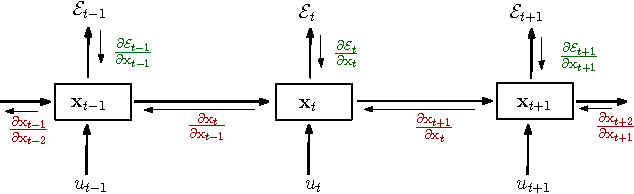
\includegraphics[width=0.8\textwidth]{BPTT}
	\caption[Minh họa thuật toán Back propagation through time]{Tại mỗi bước thời gian $t$, đội lỗi không chỉ được lan truyền qua các tầng ở bước thời gian hiện tại mà còn phải lan truyền thông tin độ lỗi qua tất cả thời điểm trước đó. Chính sự lan truyền qua thời gian này gây ra hiện tượng bùng nổ hoặc biến mất gradient.}
	\label{fig_BTT}
\end{figure}

Nhắc lại rằng trong RNN, gradient của hàm lỗi tại bước thời gian $t$ theo tham số hồi quy $\theta  \in \{W_{hh}, W_{xh}, b_h \}$ là:
\begin{equation} \label{beginGradientVanish0}
\nabla_{\theta}L_t = \frac{\partial L_t}{\partial s_t} \frac{\partial s_t}{\partial h_t} \sum_{r=0}^{t}  \frac{\partial h_t}{\partial h_r}\frac{\partial h_r}{\partial \theta}
\end{equation}
và 
\begin{equation} \label{beginGradientVanish1}
\frac{\partial h_t}{\partial h_r} = \prod_{i=r}^{t} W_{hh}^T \diag \left( \phi'(h_i) \right)
\end{equation}

Đầu tiên, để cho đơn giản, ta hãy xem $\phi$ là hàm một hàm đồng nhất (identity function) với $\phi(x) = x$ như vậy theo công thức trên, ta có:
\begin{equation} \label{gradientVanish3}
\frac{\partial h_t}{\partial h_r} = \prod_{i=r}^{t} W_{hh}^T = \left (W_{hh}^T \right)^{t-r}
\end{equation}

Với $W_{hh}$ là một ma trận vuông, nó có thể được phân tích thành dạng:
\begin{equation} \label{gradientVanish4}
W_{hh} = \Sigma \diag \left(\lambda \right) \Sigma^{-1} 
\end{equation}

Với $\Sigma, \lambda$ lần lượt là ma trận véc-tơ riêng và véc-tơ trị riêng của ma trận $W_{hh}$. Ta biết rằng lũy thừa của $W_{hh}$ cũng chính là lũy thừa của véc-tơ trị riêng của nó $\lambda$. Khi số mũ của phép lũy thừa lớn, những véc-tơ riêng ứng với trị riêng $\lambda_i < 1$ sẽ giảm theo hàm mũ, những véc-tơ riêng ứng với trị riêng $\lambda_i > 1$ sẽ tăng theo hàm mũ. Nói cách khác, \textit{điều kiện đủ} để xảy ra gradient biến mất là trị riêng lớn nhất của ma trận kết nối hồi quy $\lambda_{max}$ có giá trị nhỏ hơn 1. Để xảy ra gradient bùng nổ, \textit{điều kiện cần} là $\lambda_{max} > 1$.

Trong trường hợp tổng quát với một hàm kích hoạt $\phi$ bất kỳ, với $\phi'$ bị chặn trên bởi $\gamma \in \mathbb{R}$ và do đó $||diag(\phi'(h_k))|| \leq \gamma$. Với $\lambda_{max} < \frac{1}{\gamma}$, hiện tượng gradient biến mất sẽ xảy ra. Theo công thức \ref{gradientWRTSt16}:
\begin{equation} \label{gradientVanish5}
\forall i, \norm{\frac{\partial h_{i+1}}{\partial h_{i}}} \leq \norm{ W^T_{hh} } \norm{ diag(\phi'(h_k)) } < \frac{1}{\gamma} \gamma < 1 
\end{equation}

Đặt $\beta \in \mathbb{R}$ sao cho $\forall i, \norm{\frac{\partial h_{i+1}}{\partial h_{i}}} \leq \beta < 1$, như vậy ta có thể thấy được rằng:
\begin{equation} \label{gradientVanish6}
\lim_{t - r \to \infty} \frac{\partial h_{t}}{\partial h_r} = \prod_{i=r}^{t} W_{hh}^T \diag \left(\phi'(h_i) \right) \leq \beta^{t - r} = 0
\end{equation}

Bằng cách đảo ngược chứng minh này ta được \textit{điều kiện cần} để xảy ra gradient bùng nổ là trị riêng lớn nhất $\lambda_{max}$ lớn hơn $\frac{1}{\gamma}$.

Chứng minh trên cho thấy rằng, khi $t-r$ lớn, tức là khoảng cách giữa từ đang xét và một từ trong quá khứ là lớn thì $\nabla_{\theta_r} L_t$ sẽ hoặc rất bé nếu $\lambda_{max} < \frac{1}{\gamma}$ hoặc có khả năng trở nên rất lớn nếu $\lambda_{max} > \frac{1}{\gamma}$. Trong thực tế, với $\phi$ là hàm \textbf{tanh} ta có $\gamma = 1$ trong khi với $\phi$ là hàm sigmoid, ta có $\gamma = 1/4$. Nếu ta khởi tạo tham số $\theta$ nhỏ hoặc dùng hàm kích hoạt có $\gamma$ nhỏ như hàm \textbf{sigmoid} thì sự biến mất gradient sẽ dễ rất dễ xảy ra; nó khiến cho mô hình chỉ học được những phụ thuộc cục bộ. Ngược lại, nếu $\theta$ được khởi tạo với giá trị lớn, gradient tại các bước thời gian ở xa sẽ bùng nổ và kết quả là mô hình không thể học được \cite{pascanu2011}.

Một kỹ thuật để đối phó với sự bùng nổ gradient được đề là chuẩn hóa gradient về một giá trị nếu nó vượt quá một ngưỡng nào đó. Kỹ thuật này gọi là \textit{gradient norm clipping} \cite{pascanu2011}. Cụ thể, ta đặt một ngưỡng là chặn trên cho gradient, tại mỗi bước thời gian $t$ trong lúc backpropagation, nếu độ lớn của gradient lớn hơn ngưỡng này ta sẽ chuẩn hóa trở về một giá trị nhỏ hơn. Giải pháp này được áp dụng trong thực tế để ngăn chặn các giá trị \textbf{NaN} (Not a Number) trong gradient và cho phép quá trình huấn luyện tiếp tục. Gradient norm clipping được trình bày trong thuật toán \ref{alg_GDClipping}.

\begin{algorithm}
	\newalgname{Thuật toán}
	\caption{Gradient clipping}
	\label{alg_GDClipping}
	\begin{algorithmic}[1]
		\renewcommand{\algorithmicrequire}{\textbf{Đầu vào:}}
		\renewcommand{\algorithmicensure}{\textbf{Đầu ra:}}
		\algnewcommand\algorithmicoperation{\textbf{Thao tác:}}
		\algnewcommand\Operation{\item[\algorithmicoperation]}
		
		\Require Gradient ứng với tham số $\theta$
		\Ensure Gradient ứng với tham số $\theta$ được chuẩn hóa về một ngưỡng $threshold$
		
		\Operation
		\State $\hat{g} \leftarrow \frac{\partial E}{\partial \theta}$
		\If {$\norm{\hat{g}} \geq threshold$}
		\State $\hat{g} \leftarrow \frac{threshold}{\norm{\hat{g}}} \hat{g}$
		\EndIf
	\end{algorithmic}
\end{algorithm}

Mặt khác, vấn đề biến mất gradient là khó giải quyết hơn. Đã có nhiều cách tiếp cận được đề xuất để giải quyêt vấn đề này như \textit{Hessian Free Optimization} \cite{martens2011}, \textit{Echo State Network} \cite{jaeger2007}, \textit{Long short-term memory} \cite{hochreiter1997} và một số phương pháp khác được liệt kê trong \cite{bengio2013}. Trong số những phương pháp đó, Long short-term memory (LSTM) là phương pháp thường được sử dụng nhất. LSTM là phiên bản nâng cấp của RNN với các chê chế để giải quyết hiệu quả vấn đề biến mất gradient, hơn thế nữa, với các cơ chế của mình, LSTM còn có thể giải quyết vấn đề bùng nổ gradient và giúp mạng nơ-ron hồi quy học tốt hơn. Nó cũng chính là phiên bản mạng nơ-ron hồi quy mà chúng tôi sử dụng trong khóa luận này. Trong phần tiếp theo, chúng tôi sẽ trình bày về LSTM và giải thích vì sao LSTM hiệu quả không chỉ trong việc giải quyết vấn đề biến mất gradient mà còn cho cả vấn đề bùng nổ gradient và mất mát thông tin.

\section{Long short-term memory (LSTM)}

\begin{figure}
	\centering
	\includegraphics[width=0.7\textwidth]{LSTMcell}
	\caption[Một LSTM cell]{Một LSTM cell với cổng quên, ô với ký hiệu $\sigma$ đại diện cho những nút; các ô với ký hiệu $\prod$ đại diện cho các cổng. Ô tròn ở trung tâm đại diện cho trạng thái lưu giữ.}
	\label{fig_lstmCell}
\end{figure}

Hochreiter và Schmidhuber \cite{hochreiter1997} đã giới thiệu mô hình \textit{Long short-term memory} (LSTM) chủ yếu ở để khắc phục vấn đề biến mất gradient trong RNN. Nhớ lại rằng trong RNN, chính việc mô hình hóa phụ thuộc thời gian dựa vào ma trận trọng số $W_{hh}$ đã gây ra hiện tượng gradient biến mất. Giả sử gọi $S_t$ là trạng thái liên kết hồi quy (trong RNN, nó chính là trạng thái ẩn). Ý tưởng của LSTM là thay vì tính toán $S_t$ từ $S_{t-1}$ với một phép nhân ma trận theo sau là hàm kích hoạt phi tuyến, LSTM trực tiếp tính toán một $\Delta S_t$ sau đó nó được cộng với $S_{t-1}$ để tạo ra $S_t$. Thoạt nhìn, sự khác biệt này có thể không đáng kể khi mà $S_t$ đều đạt được trong cả hai cách. Tuy nhiên, với cách làm này, các gradient của LSTM tính toán $\Delta S_t$ sẽ không bị biến mất.

Thuật ngữ "Long short-term memory" xuất phát từ nhận định sau. Mạng RNN đơn giản có "long term memory" (bộ nhớ dài hạn) dưới dạng các ma trận trọng số. Những ma trận trọng số này thay đổi một cách chậm rãi trong quá trình học nhằm mã hóa kiến thức về dữ liệu. RNN cũng có "short-term memory" (bộ nhớ ngắn hạn) dưới dạng các kích hoạt tạm thời, được truyền từ mỗi bước thời gian sang các bước thời gian sau đó. "Long short-term memory" tạm dịch là "bộ nhớ ngắn hạn dài" cho phép mở rộng bộ nhớ ngắn hạn bằng cách thêm vào một loại lưu trữ trung gian gọi là trạng thái lưu giữ (cell state). Trạng thái lưu giữ này có khả năng lưu giữ các thông tin cần thiết một cách lâu dài dưới dạng một bộ nhớ ngắn hạn. Để làm được điều này, LSTM sử dụng một cơ chế gọi là "cổng", các "cổng" giúp được huấn luyện để chọn lọc thông tin nào là cần thiết để tác động lên trạng thái lưu trữ. Với cách làm này, trạng thái lưu trữ sẽ lưu được nhiều thông tin hơn, vì chỉ những thông tin quan trọng mới tồn tại trong nó.

Về cấu tạo, một LSTM tương tự như một RNN một lớp ẩn, nhưng mỗi RNN cell (ký hiệu "A" trong hình \ref{fig_rnn_unrolled}) được thay thế bằng một \textit{memory cell} (hình \ref{fig_lstmCell}). Giống như RNN cell, memory cell nhận một đầu vào bên ngoài và phát sinh một đầu ra cũng như là truyền đi một trạng thái ẩn sang memory cell ở bước thời gian kế tiếp. Tuy nhiên, trong memory cell còn có thêm một trạng thái lưu giữ cũng được truyền đi như một trạng thái ẩn. Cấu tạo chi tiết của LSTM sẽ được trình bày trong phần dưới đây, cấu tạo này dựa trên phiên bản LSTM của \cite{gers2000}.

\begin{itemize}
	\item[•] \textit{Nút đầu vào (input node)}: Đơn vị này được ký hiệu là $g$, là một mạng nơ-ron một tầng ẩn. Nút đầu vào có nhiệm vụ mô hình hóa đầu vào tại mỗi bước thời gian. Nó nhận tham số là đầu vào tại bước thời gian hiện tại $x_t$ và trạng thái ẩn tại thời điểm trước đó $h_{t-1}$. Cụ thể, tại mỗi bước thời gian nút đầu vào có công thức:
	\begin{equation} \label{inputNodeLSTM}
	g_t = \phi \left(W_{gx}x_t + W_{gh}h_{t-1} + b_g \right)
	\end{equation}
	\item[•] \textit{Cổng vào (input gate)}: "Cổng" như đã nói, là một cơ chế đặc biệt của LSTM. Cổng vào cũng được cấu tạo giống như nút đầu vào, nó nhận tham số là $x_t$ và $h_{t-1}$. Sau đó được đưa qua hàm kích hoạt $\sigmoid$ để tạo ra giá trị trong khoảng $(0,1)$. Sở dĩ đơn vị này được gọi là "cổng vào" vì giá trị của nó sẽ được sử dụng để nhân với giá trị của nút đầu vào. Giá trị của nó thể hiện lượng thông tin mà nút đầu vào được phép truyền đi. Nếu cổng vào bằng 0, nút đầu vào sẽ truyền đi với giá trị 0. Nếu cổng vào bằng 1, nút đầu vào sẽ truyền đi với giá trị ban đầu. Cụ thể hơn, ta có công thức của cổng vào, được ký hiệu là $i$, tại bước thời gian $t$:
	\begin{equation} \label{inputGateLSTM}
	i_t = \sigma \left(W_{ix}x_t + W_{ih}h_{t-1} + b_i \right)
	\end{equation}
	\item[•] \textit{Trạng thái lưu giữ (cell state)}: Trái tim của LSTM chính là trạng thái lưu trữ, là một mạng nơ-ron với hàm kích hoạt tuyến tính. Khá giống với trạng thái ẩn trong RNN, trạng thái lưu trữ $s_t$ cũng có một kết nối hồi quy với trạng thái lưu trữ trước đó $s_{t-1}$. Tuy nhiên, trọng số kết nối hồi quy luôn có giá trị cố định là 1. Bởi vì kết nối hồi quy này qua nhiều bước đều có trọng số không đổi nên khi tính toán, gradient của độ lỗi không bị bùng nổ hay biến mất. Tại mỗi bước thời gian, trạng thái lưu trữ được tính như sau:
	\begin{equation} \label{cellStateLSTM}
	s_t = s_{t-1} + g_t \odot i_t
	\end{equation}
	ký hiệu $\odot$ nghĩa là phép nhân theo từng phần tử (element-wise multiplication).
	\item[•] \textit{Cổng quên (forget gate)}: Cổng quên là một đề xuất của \cite{gers2000} so với bài báo LSTM gốc. Thay vì kiểm soát lượng thông tin để đưa vào trạng thái lưu giữ như cổng vào, cổng quên cung cấp khả năng tẩy đi một lượng thông tin trong trạng thái lưu giữ. Cụ thể, cổng quên với giá trị thuộc khoảng $(0,1)$ sẽ được nhân với $s_{t-1}$ trong công thức \ref{cellStateLSTM}. Tại mỗi bước thời gian, giá trị của cổng quên $f_t$ được tính như sau:
	\begin{equation} \label{forgetGateLSTM}
	f_t = \sigma \left(W_{fx}x_t + W_{fh}h_{t-1} + b_f \right)
	\end{equation}
	Công thức của trạng thái lưu trữ được sửa lại khi có cổng quên:
	\begin{equation} \label{cellStateWithForgetGateLSTM}
	s_t = s_{t-1} \odot f_t + g_t \odot i_t
	\end{equation}
	\item[•] \textit{Cổng ra (output gate)}: Giá trị đầu ra $v_t$ của memory cell tại mỗi bước thời gian chính là tích giá trị của trạng thái lưu trữ $s_t$ với giá trị của cổng ra $o_t$. Trong một số phiên bản của LSTM, hàm kích hoạt $\phi$ có thể là hàm \textbf{tanh} hoặc \textbf{sigmoid} hoặc không sử dụng hàm kích hoạt nào. Tại mỗi bước thời gian, giá trị của cổng ra $o_t$ được tính như sau:
	\begin{equation} \label{outputGateLSTM}
	o_t = \sigma \left(W_{ox}x_t + W_{oh}h_{t-1} + b_o \right)
	\end{equation}
	Đầu ra của memory cell cũng chính là trạng thái ẩn $h_t$ có giá trị:
	\begin{equation} \label{outputNodeLSTM}
	h_t = \phi(s_t) \odot o_t 
	\end{equation}
\end{itemize}

Như đã phân tích, đối với RNN, trạng thái ẩn được tạo ra một cách trực tiếp từ trạng thái ẩn trước đó thông qua phép biến đổi phi tuyến. Điều này làm cho gradient bị biến mất trong quá trình lan truyền ngược từ trạng thái ẩn này sang trại thái ẩn khác. Trong khi đó, với LSTM, trạng thái ẩn được tính một cách gián tiếp thông qua trạng thái lưu giữ mà những trạng thái lưu trữ này được kết nối với nhau qua một phép biến đổi tuyến tính. Điều này giúp cho gradient không bị thay đổi trong quá trình lan truyền ngược. Do đó giảm khả năng LSTM gặp phải vấn đề gradient bị biến mất hay bùng nổ. Ngoài ra, với cơ chế cổng, LSTM có khả năng chọn lọc những thông tin cần thiết, loại bỏ các thông tin thừa trong trạng thái ẩn, điều này giúp tăng khả năng lưu trữ thông tin so với RNN. Ta thấy rằng nếu muốn lấy thông tin từ một thời điểm nào đó, LSTM có thể học để đóng các cổng đầu vào và cổng quên, cho nên thông có thể truyền từ một thời điểm đi rất xa mà ít bị mất mát (hình \ref{fig_infoconst} thể hiện khả năng bảo vệ thông tin của LSTM). Khả năng bảo quản thông tin tốt và nắm bắt các phụ thuộc dài hạn chính là lý do vì sao LSTM được chọn để làm bộ mã hóa và bộ giải mã trong khóa luận này.

\begin{figure}
	\centering
	\includegraphics[width=0.85\textwidth]{infoconst}
	\caption[Minh họa quá trình thông tin dài hạn trong LSTM được duy trì]{Minh họa quá trình thông tin dài hạn trong LSTM được duy trì. Hình vẽ này minh họa cách thông tin của đầu vào tại thời điểm thứ nhất được duy trì một cách toàn vẹn khi lan truyền qua các thời điểm tiếp theo; màu càng đậm tương ứng với lượng thông tin của đầu vào thứ nhất càng nhiều. Ở đây, mỗi nơ-ron ẩn có các cổng: cổng quên (bên trái), cổng vào (bên dưới) và cổng ra (bên trên) của các trạng thái ẩn; một cổng mở hoàn toàn được kí hiệu bởi “$\circ$”, và đóng hoàn toàn được kí hiệu bởi “$-$”. Để duy trì thông tin của đầu vào thứ nhất một cách toàn vẹn, tại tất cả các thời điểm, các cổng xóa được mở hoàn toàn để lấy toàn bộ thông tin của đầu vào thứ nhất; trong khi đó, từ thời điểm thứ hai, các cổng đầu vào đóng hoàn toàn để chặn thông tin của các đầu vào mới. Tại thời điểm nào mà trạng thái ẩn cần sử dụng tất cả thông tin của đầu vào thứ nhất, mô hình chỉ cần mở hoàn toàn cổng đầu ra để lấy toàn vẹn thông tin này.}
	\label{fig_infoconst}
\end{figure}

%\subsection{Huấn luyện mạng LSTM}
%Quá trình huấn luyện mạng LSTM cũng giống như quá trình huấn luyện RNN vì những thành phần cấu tạo nên chúng hầu giống hệt nhau. Một điểm khác biệt là cơ chế hồi quy trong RNN sử dụng $h$ là thành phần hồi quy duy nhất. Trong LSTM, cả $h$ và $c$ đều được sử dụng làm thành phần hồi quy:
%\begin{equation} \label{lstmrecurrence}
%	\left(h_t, c_t \right) = f \left(x_t, h_{t-1}, c_{t-1} \right)
%\end{equation}


\subsection{Mạng nơ-ron hồi quy hai chiều}

Trong một số trường hợp, tại một bước thời gian, để dự đoán kết quả của mạng nơ-ron hồi quy, mô hình không chỉ cần các thông tin ngữ cảnh từ quá khứ mà còn cần những thông tin ngữ cảnh từ tương lai. Ví dụ như trong bài toán gán nhãn từ loại (part-of-speech tagging): ta cần gán từ loại cho mỗi từ trong câu $w_i$, nếu sử dụng một RNN đơn thuần, mô hình sẽ chỉ sử dụng được những thông tin từ những từ phía trước $w_1,...,w_{i-1}$ để dự đoán nhãn của từ $w_i$, sẽ hiệu quả hơn nếu tận dụng được cả những từ phía sau $w_{i+1},...,w_{N}$ cho việc dự đoán. Việc này không thể thực hiện được chỉ với mạng nơ-ron hồi quy đơn thuần. 

Công trình \cite{schuster1997} đề xuất mô hình mạng nơ-ron hồi quy hai chiều (Bidirectional recurrent neural network). Mô hình này rất giống mạng nơ-ron hồi quy được trình bày trong mục \ref{rnnsection} ngoại trừ việc tại mỗi bước thời gian $t$, mô hình này duy trì hai lớp ẩn (thay vì một như trong RNN thông thường): một lớp ẩn được truyền từ trái sang phải và một truyền từ phải sang trái. Hai lớp ẩn này tương đương với hai véc-tơ trạng thái ẩn, trạng thái ẩn tổng hợp tại mỗi bước thời gian là véc-tơ nối dài của hai trạng thái ẩn này. Có thể coi RNN hai chiều là hai RNN độc lập nhau trừ việc chúng sử dụng cùng một đầu ra và bộ các tham số. Có thể diễn tả một RNN hai chiều bằng công thức:

\begin{align}
\overleftarrow{h_t} &= \phi \left(W_{xh} x_{t} + W_{hh} h_{t-1} + b_h \right) \\ \label{birnn1} 
\overrightarrow{h_t} &= \phi \left(W_{xh} x_{t} + W_{hh} h_{t+1} + b_h \right) \\ \label{birnn2}
\hat{y}_t &= \zeta \left(W_{hy} \left[\overleftarrow{h_t}; \overrightarrow{h_t} \right] + b_y \right) \\ \label{birnn3}	 \nonumber
\end{align}
trong công thức trên, $\overleftarrow{h_t}, \overrightarrow{h_t}$ lần lượt là véc-tơ trạng thái ẩn truyền từ phải sang trái và từ trái sang phải. $\zeta$ là một hàm đầu ra (như hàm $\softmax$).

\begin{figure}
	\centering
	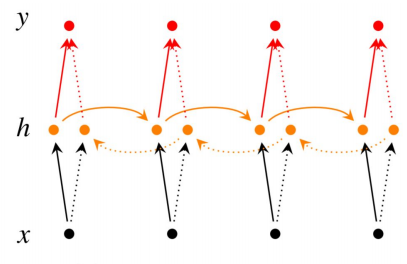
\includegraphics[width=0.7\textwidth]{birnn}
	\caption[Minh họa một bi-LSTM được dùng làm bộ mã hóa]{Minh họa một bi-LSTM được dùng làm bộ mã hóa. Trại thái ẩn cuối cùng (véc-tơ cao nhất trong hình) là sự kết hợp theo chiều dọc của hai véc-tơ trại thái ẩn cuối cùng ở hai chiều từ trái sang phải và từ phải sang trái. Nếu thay LSTM trong hình bằng RNN, ta sẽ có một bi-RNN.}
	\label{fig_birnn}
\end{figure}

Ở bước lan truyền tiến, lớp ẩn thứ nhất được kích hoạt để truyền từ trái sang phải, trong quá trình đó, những trạng thái ẩn $\overrightarrow{h_t}$ được lưu trữ lại. Sau đó, lớp ẩn thứ hai được kích hoạt để truyền từ phải sang trái và những trạng thái ẩn $\overleftarrow{h_t}$ cũng được lưu trữ lại. Cuối cùng, thực hiện lan truyền tiến ở các bước đầu ra, sử dụng trạng thái ẩn là véc-tơ nối dài của các cả hai trạng thái ẩn $\overrightarrow{h_t}$ và $\overleftarrow{h_t}$. Tương tự như vậy, ở bước lan truyền ngược, gradient ở các đầu ra được tính trước và các gradient ở đầu ra được lưu trữ lại. Sau đó, lần lượt thực hiện lan truyền ngược theo chiều từ trái sang phải và từ phải sang trái với các giá trị gradient ở đầu ra đã được lưu lại.

Mặc dù RNN hai chiều giúp tăng cường thông tin cho trạng thái ẩn ở cả hai chiều của câu, tuy nhiên nó có hai nhược điểm, một là: quá trình lan truyền tiến và lan truyền ngược ở hai chiều phải thực hiện tuần tự nhau, việc này làm chập quá trình học. Hai là: RNN hai chiều chỉ thích hợp cho những bài toán thực hiện trên dữ liệu đầy đủ, ví dụ bài tóan phân tích ý kiến (sentiment analysis), gán nhãn từ loại (part-of-speech tagging),... Đối với những bài toán mà dữ liệu chưa hoàn chỉnh, ví dụ như dự đoán từ tiếp theo trong chuỗi, việc sử dụng RNN hai chiều là bất khả thi (vì ta cần một chiều ngược lại trong bước dự đoán, cái mà chưa xảy ra).

Mô hình hai chiều cũng có thể dễ dàng áp dụng lên LSTM (thay vì RNN) với các thiết lập tương tự. Để dễ dàng trong việc gọi tên các mô hình một chiều và hai chiều. Từ đoạn này trở đi, chúng tôi ký hiệu RNN hay LSTM một chiều lần lượt là \textit{uni-RNN} và \textit{uni-LSTM}, tiền tố \textit{uni} đại diện cho \textit{unidirectional} có nghĩa là \textit{một chiều}. Tương tự như vậy RNN hay LSTM hai chiều lần lượt được ký hiệu là \textit{bi-RNN} và \textit{bi-LSTM}, tiền tố \textit{bi} đại diện cho \textit{bidirectional} có nghĩa là \textit{hai chiều}. Hình \ref{fig_birnn} mô tả một bi-LSTM trong quá trình đọc một câu nguồn.





